\chapter{Recommender Systems}
    Un $\textbf{Recommender System}$ è un sistema di filtraggio delle informazioni che fornisce suggerimenti per gli elementi più pertinenti per un particolare utente (es: film o serie tv suggerite da Netflix).
    
    \section{Misure di Qualità}
        Prima di illustrare i sistemi di raccomandazioni, bisogna fare mente locale su cosa ci serve per capire i vantaggi e svantaggi dei vari sistemi.
        \\[1\baselineskip]
        Per capire ciò, ci si avvale delle $\textit{misure di qualità}$ di un sistema di raccomandazioni.
        Tali misure sono:
            \begin{itemize}
                \item Efficienza nella costruzione del modello;
                \item Efficienza nella generazione dei suggerimenti;
                \item "Serendipity" delle raccomandazioni, ovvero abilità nel suggerire cose non banali e interessanti;
                \item Adattamento al problema della "partenza a freddo" (Cold-Start Problem).
            \end{itemize}

    \section{Sistemi}
        Possiamo identificare ben 3 tipi di recommender systems che utilizzano, ognuno, delle strategie diverse.
        \\
        Prima di tutto, denotando l'insieme degli utenti come $U$ e l'insieme degli items come $I$, formulare il profilo dell'utente $u \in U$ come:
            $$ u = \frac{1}{|I_{u}|} \cdot \sum_{x \in I_{u}}{x}$$

        \subsection{Content-Based}
            Il filtraggio basato sul contenuto utilizza le features degli items per consigliare altri items simili a quelli che piacciono all'utente, in base alle azioni precedenti o al feedback esplicito.
            \\[1\baselineskip]
            La misura di similarità che questo sistema utilizza è il coseno tra due vettori:
                $$ \cos(u, x) = \frac{u \cdot x}{\|u\| \cdot \|x\|} = \frac{\sum_{t}{u[t] \cdot x[t]}}{\sqrt{\sum_{t}{u[t]^{2}}} \cdot \sqrt{\sum_{t}{x[t]^{2}}}} $$

            dove:
                \begin{itemize}
                    \item Ogni item $x \in I$ è un vettore di dimensione $n$, con $n$ che rappresenta il numero di parole nel lessico (creatosi dopo lo stemming, lemming, etc...);
                    \item $x[t] = tf(t, x) \cdot idf(t)$;
                        \\[0.5\baselineskip]
                        $\textbf{Reminder:}$ $\textbf{tf}(t,x)$ è la frequenza del termine $t$ nell'item $x$ e $idf(t)$ è l'invero della frequenza di $t$ nell'insieme di items $I$.
                \end{itemize}

            \subsubsection{Qualità}
                \begin{itemize}
                    \item Facile da costruire in quanto la costruzione di un vettore per ciascuno item non è tanto costoso;
                    \item Non è efficiente nella generazione dei suggerimenti siccome deve cercare i vicini più "vicini" tra tutti i documenti;
                    \item Poca serendipity proprio perché è legato alla similarità del testo di un item;
                    \item Cold-Start Problem "parziale" in quanto un utente dovrebbe prima "toccare" almeno un item.
                \end{itemize}

        \subsection{User-Based}
            Il filtraggio basato sull'utente è una tecnica utilizzata per prevedere gli elementi che potrebbero piacere a un utente sulla base delle valutazioni assegnate a tale elemento dagli altri utenti che hanno gusti simili a quelli dell'utente target.
            \\[1\baselineskip]
            Utilizza una misura di similarità basata su un $\textbf{ranking score}$ $s_{ui}$ dove $u \in U$ e $i \in I$ (indica lo score dell'item $i$ per l'utente $u$):
                $$ s_{ui} = \frac{\sum_{v \in N(u)}{(v[i] - \overline{v}) \cdot \rho(u,v)}}{\sum_{v \in N(u)}{|\rho(u,v)|}} $$

            dove:
                \begin{itemize}
                    \item $\rho(u,v)$ è il $\textbf{coefficiente di correlazione di Pearson}$, usato per pesare il rating di ogni utente $v \in N(u)$ per la similarità tra $v$ e $u$;
                    \item $N(u)$ sono i vicini dell'utente $u$, ovvero un set di utenti simili all'utente target $u$;
                \end{itemize}

            È possibile predire il rating da parte dell'utente $u$ come: $r_{ui} = \overline{u} + s_{ui}$.

            \subsubsection{Qualità}
                \begin{itemize}
                    \item Costoso da costruire in quanto il calcolo della similarità per ogni utente è molto costosa ($O(|U|^{2})$) e deve essere ricomputata per ogni nuovo rating di un utente;
                    \item Efficiente nella generazione dei suggerimenti se la ricerca dei "vicini" viene precomputata offline;
                    \item Ottima serendipity;
                    \item Il Cold-Start Problem è molto problematico perché ha bisogno di un set di ratings sufficientemente grande per ogni nuovo utente/item.
                \end{itemize}

        \subsection{Item-based}
            Il filtraggio basato sull'elemento cerca elementi simili in base agli elementi che gli utenti hanno precedentemente apprezzato o con cui hanno precedentemente interagito positivamente e li consiglia di conseguenza.
            \\[1\baselineskip]
            Utilizza la misura di similarità del coseno, ma aggiustata in modo tale che la misura sia diversa se il set di ratings è diverso
                $$ a-cos(i,j) = \frac{\sum_{u}{(i[u] - \overline{u}) (j[u] - \overline{u})}}{\sqrt{\sum_{u}{(i[u] - \overline{u})^{2}}} \cdot \sqrt{\sum_{u}{(j[u] - \overline{u})^{2}}}} $$

            $\textbf{Nota:}$ il coseno "normale" non è influenzato dalla scala degli elementi/utenti, quindi è come se fossero tutti sulla stessa scala.
                \begin{figure}[h]
                    \caption{A e B sono molto simili ma A è valutato peggio!}
                    \centering
                    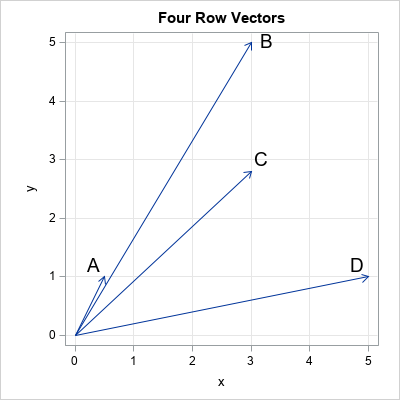
\includegraphics[width = 8cm, height = 6.5cm]{cosine-example.png}
                \end{figure}

            \subsubsection{Qualità}
                \begin{itemize}
                    \item Efficiente da costruire in quanto le computazioni avvengono offline e, generalmente, $|I|$ e più piccolo di $|U|$;
                    \item Efficiente nella generazione dei suggerimenti visto che la ricerca dei vicini più vicini non è necessaria se precomputata offline;
                    \item Meno di quella dello User-Based, siccome il ranking finale dipende dalle ratings dell'utente corrente;
                    \item Il Cold-Start Problem è molto problematico perché ha bisogno di un set di ratings sufficientemente grande per ogni nuovo utente/item.
                \end{itemize}

\clearpage